% Compact PGFPlots panel for sampled surface15 BSC bit-scale decomposition.
% Requires \usepackage{pgfplots} and \pgfplotsset{compat=1.18}.
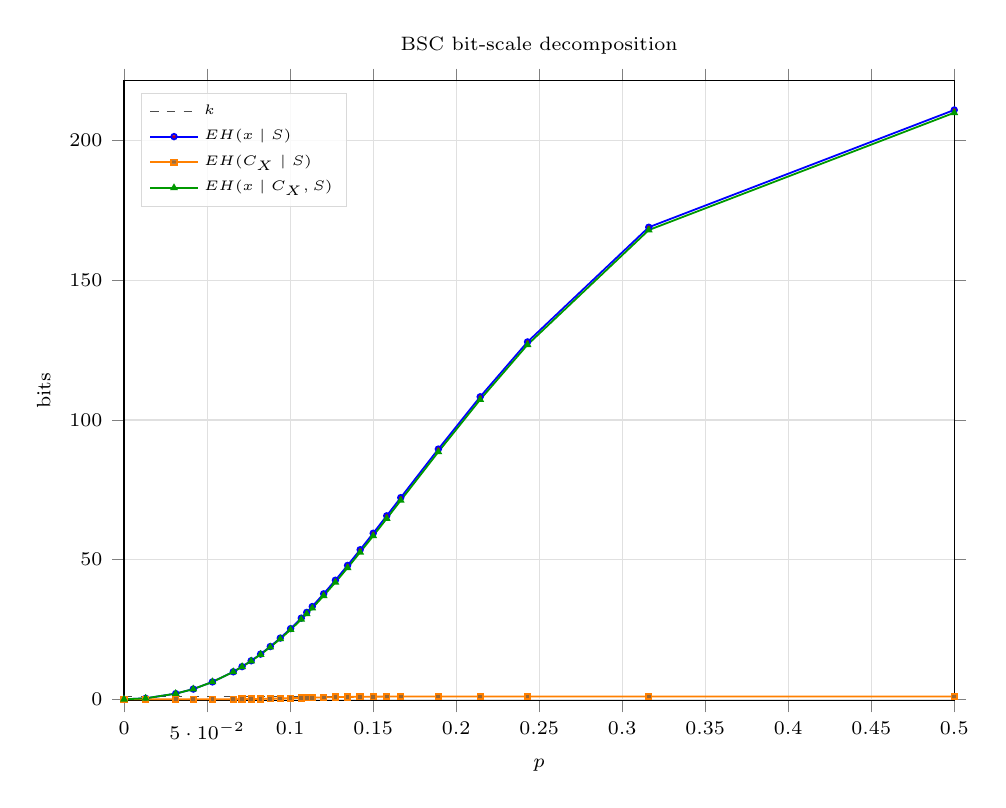
\begin{tikzpicture}
\begin{axis}[
  name=Surface15BSCBitScaleAxis,
  width=\linewidth,
  height=0.78\linewidth,
  title={BSC bit-scale decomposition},
  title style={font=\scriptsize},
  xlabel={$p$},
  ylabel={bits},
  xmin=0, xmax=0.5,
  ymin=-0.5, ymax=221.55,
  grid=both,
  major grid style={black!12},
  minor grid style={black!6},
  tick align=outside,
  tick label style={font=\scriptsize},
  label style={font=\scriptsize},
  legend cell align={left},
  legend style={draw=black!15, fill=white, fill opacity=0.82, text opacity=1, at={(0.02,0.98)}, anchor=north west, font=\tiny},
]
\addplot[black!70, dashed, line width=0.55pt] coordinates {(0,1) (0.5,1)};
\addlegendentry{$k$}
\addplot+[color=blue, mark=*, mark size=1.0pt, line width=0.65pt]
coordinates {(0,0) (0.0129868620555,0.336190415026) (0.0311244603048,2.01736699343) (0.0416926902737,3.65333778016) (0.0532390407768,6.21052804697) (0.0657867063546,9.83357143318) (0.0710958755299,11.694485812) (0.0765765344037,13.7867570095) (0.0822333323659,16.1719559075) (0.0880715694979,18.8781174355) (0.0940972433461,21.9089925667) (0.100317108961,25.2889525364) (0.106738753821,29.0499755817) (0.110027864438,31.0976067696) (0.113370689941,33.199530795) (0.120222466333,37.7556013263) (0.127304805976,42.6254660713) (0.134629772869,47.9181331578) (0.142210976498,53.5460376858) (0.150063823499,59.4479119559) (0.158205829694,65.6788337527) (0.166657010397,72.19010917) (0.189297705371,89.5803696299) (0.21450174486,108.298742687) (0.243003853809,127.945628092) (0.316019346324,169.003946601) (0.5,211)};
\addlegendentry{$\mathbb{E}H(x\mid S)$}
\addplot+[color=orange, mark=square*, mark size=1.0pt, line width=0.65pt]
coordinates {(0,0) (0.0129868620555,1.42409912011e-12) (0.0311244603048,3.3435160352e-06) (0.0416926902737,0.00190982850045) (0.0532390407768,0.00724084226435) (0.0657867063546,0.0330010237808) (0.0710958755299,0.0579094461663) (0.0765765344037,0.0912368711581) (0.0822333323659,0.13763989118) (0.0880715694979,0.204324101433) (0.0940972433461,0.281663627662) (0.100317108961,0.370692229197) (0.106738753821,0.474927930676) (0.110027864438,0.529606033742) (0.113370689941,0.582364187184) (0.120222466333,0.679049301224) (0.127304805976,0.760873710735) (0.134629772869,0.838963390557) (0.142210976498,0.901076335766) (0.150063823499,0.938537611163) (0.158205829694,0.966346465547) (0.166657010397,0.982759036129) (0.189297705371,0.997566510793) (0.21450174486,0.999736765159) (0.243003853809,0.999993993881) (0.316019346324,0.999999997119) (0.5,1)};
\addlegendentry{$\mathbb{E}H(C_X\mid S)$}
\addplot+[color=green!60!black, mark=triangle*, mark size=1.0pt, line width=0.65pt]
coordinates {(0,0) (0.0129868620555,0.336190415025) (0.0311244603048,2.01736364991) (0.0416926902737,3.65142795166) (0.0532390407768,6.2032872047) (0.0657867063546,9.8005704094) (0.0710958755299,11.6365763659) (0.0765765344037,13.6955201383) (0.0822333323659,16.0343160163) (0.0880715694979,18.6737933341) (0.0940972433461,21.627328939) (0.100317108961,24.9182603072) (0.106738753821,28.575047651) (0.110027864438,30.5680007358) (0.113370689941,32.6171666078) (0.120222466333,37.0765520251) (0.127304805976,41.8645923606) (0.134629772869,47.0791697672) (0.142210976498,52.64496135) (0.150063823499,58.5093743447) (0.158205829694,64.7124872872) (0.166657010397,71.2073501339) (0.189297705371,88.5828031191) (0.21450174486,107.299005922) (0.243003853809,126.945634098) (0.316019346324,168.003946604) (0.5,210)};
\addlegendentry{$\mathbb{E}H(x\mid C_X,S)$}
\end{axis}
\end{tikzpicture}
